
\documentclass[a4paper]{article}

\usepackage{amsmath,amssymb,latexsym, marvosym}
\usepackage{tikz}
\usetikzlibrary{shapes,snakes}

\begin{document}

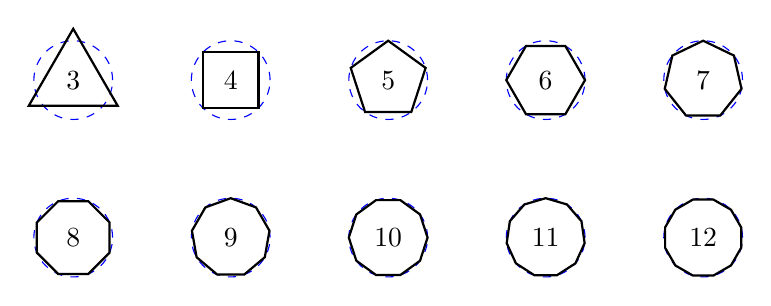
\begin{tikzpicture}

% Define box and box title style
\tikzstyle{ngon} =[regular polygon, 
                   draw, thick, minimum size = 1cm]

\foreach \a in {3,...,7}{
  \draw[blue, dashed] (\a*2,0) circle(0.5cm);
  \node[ngon, regular polygon sides=\a] at (\a*2, 0) {$\a$};
}
\foreach \a in {8,...,12}{
  \draw[blue, dashed] (\a*2 -10 ,-2) circle(0.5cm);
  \node[ngon, regular polygon sides=\a] at (\a*2 -10 , -2) {$\a$};
}


\end{tikzpicture}%


\end{document}
